\documentclass[conference]{IEEEtran}
\IEEEoverridecommandlockouts
\usepackage{cite}
\usepackage{amsmath,amssymb,amsfonts}
\usepackage{algorithmic}
\usepackage{graphicx}
\usepackage{textcomp}
\usepackage{xcolor}
\usepackage{booktabs}
\usepackage{microtype}
\usepackage{url}

\begin{document}

\title{BioDINO-Edge: Biologically-Grounded Multimodal Few-Shot Learning for Ultra-Fast Crop Pathology on Resource-Constrained Micro-Scouts}

\author{
    \IEEEauthorblockN{Reyhane Javidi Alsaadi}
    \IEEEauthorblockA{\textit{Department of Computer Engineering} \\
    \textit{Dr. Shariaty Technical University} \\
    Tehran, Iran \\
    reyhane.code@gmail.com}
    \and
    \IEEEauthorblockN{Mohammad Reza Samad Zadeh}
    \IEEEauthorblockA{\textit{Department of Computer Engineering} \\
    \textit{Dr. Shariaty Technical University} \\
    Tehran, Iran}
}

\maketitle

\begin{abstract}
Rapid and accurate foliar disease diagnosis is vital for global food security, yet existing deep learning paradigms fall short of practical agricultural deployment. Deep convolutional networks demand thousands of curated field images per pathology, while general-purpose vision foundation models suffer from severe domain gap on foliar histology. Furthermore, gradient-based meta-learning methods incur prohibitive computational and memory footprints, precluding autonomous edge execution. To overcome these limitations, we introduce \textbf{BioDINO-Edge}, an adaptive dual-foundation framework uniting self-supervised visual embeddings (DINOv2 Small) with organismal taxonomic vision-language supervision (BioCLIP ViT-B). By coupling high-dimensional Regularized Fisher Linear Discriminant Analysis (Fisher-LDA) with closed-form Soft-Anchored Transductive Self-Calibration, BioDINO-Edge establishes an optimal foliar manifold that suppresses shared vegetative background variance by over $31\times$ and eliminates small-sample covariance singularity ($N \ll d$) via analytical Ledoit--Wolf shrinkage without backpropagation. An integrated predictive Shannon margin-entropy gate dynamically arbitrates queries: routine foliar patterns exit via the lightweight fast path in 21.1\,ms ($>$45 FPS), while ambiguous queries trigger the multimodal consensus companion. Across the 11-class PlantVillage benchmark under strict 5-shot constraints, BioDINO-Edge establishes a new state of the art with \textbf{98.72\% peak accuracy}, \textbf{98.41\% peak F1-score}, and a 30-episode mean of \textbf{97.37\% $\pm$ 0.73\%}, outperforming CLIP+LoRA by 10.66 percentage points while reducing false-negative disease escape to 0.604\%. On the uncontrolled in-the-wild PlantDoc dataset, it attains 83.61\% 5-way 5-shot accuracy ($+$13.00\% over prior SOTA) and 56.35\% in 27-way field stress testing. Compiling into a standalone 22.73\,MB native Android APK operating at sub-22\,ms latency alongside an on-demand 85.3\,MB companion, BioDINO-Edge delivers a field-ready, mathematically rigorous diagnostic capability for autonomous agricultural scouting.
\end{abstract}

\begin{IEEEkeywords}
Few-Shot Learning, Precision Agriculture, Plant Pathology, Multimodal Foundation Models, Fisher Discriminant Analysis, Edge AI, Transductive Inference.
\end{IEEEkeywords}

\section{Introduction}
Plant pests and diseases destroy an estimated 20\%--40\% of crops annually \cite{richard2022control}. Traditional plant-pathogen diagnosis depends largely on visual inspection of leaf symptoms, most commonly discoloration, abnormal shape, and lesions \cite{khakimov2022traditional}. In field practice, visual inspection is slow, depends on trained scorers, and becomes ambiguous when different pathogens produce similar lesions \cite{shoaib2023advanced}; faster and more reliable identification is therefore needed.

Deep learning provides an automated alternative for plant disease identification by learning discriminative features directly from images \cite{shoaib2023advanced}. However, conventional supervised models require large labeled datasets to achieve reliable diagnosis. Such datasets are difficult to acquire in real-world agricultural settings due to the limited availability and diversity of field images \cite{shoaib2023advanced, shafik2023systematic}.

Few-shot learning (FSL) has become a common strategy: rather than collecting thousands of labeled images, it trains a model to recognize new disease classes from a handful of support examples. Recent studies have applied FSL with cross-domain few-shot models---such as CDFSL-BDC \cite{yang2024laboratory} and MAFDE-DN4 \cite{zhao2024mafde}---as well as few-shot metric domain adaptation (FMDA) \cite{kudo2025few}, visual-semantic fusion (TSMF) \cite{zhou2026vsf}, and edge-federated approaches \cite{sharif2026real}. These approaches, however, face several practical limitations.

Cross-domain FSL models such as CDFSL-BDC \cite{yang2024laboratory} struggle with complex backgrounds and scale-varying lesions when labels are scarce, and FMDA \cite{kudo2025few} still requires some labeled target data; TSMF's \cite{zhou2026vsf} GPT-4o descriptions were only 20\% manually checked and remain class-level rather than query-specific, so fine-grained visual--semantic alignment is limited. FMEL-FSDA \cite{sharif2026real} was not evaluated with real sensor/IoT streams and its federated setup was not tested at large cross-institution scale, leaving real-time edge performance under field data unproven.

We introduce BioDINO-Edge, a gradient-free dual-foundation pipeline tailored for cross-domain few-shot plant pathology under edge constraints. Mechanistically, DINOv2 provides high-resolution spatial cues for microscopic lesion margins, BioCLIP supplies organismal taxonomic priors to eliminate cross-species semantic misalignment, and closed-form Fisher-LDA whitens shared vegetative background variance to suppress domain shift without backpropagation. While highly effective under diverse field conditions, a practical limitation is that severe optical defocus blur can degrade high-frequency lesion textures and occasionally bypass the uncertainty gate.

The key contributions of this work are as follows:
\begin{enumerate}
    \item \textbf{Dual-Foundation Foliar Representation:} Uniting self-supervised visual embeddings from DINOv2 \cite{oquab2023dinov2} with BioCLIP's \cite{stevens2024bioclip} visual and textual botanical representations to resolve subtle necrotic lesions without foundation-model fine-tuning.
    \item \textbf{Closed-Form Analytical Adaptation:} Integrating Fisher-LDA \cite{fisher1936use} with Ledoit--Wolf covariance shrinkage \cite{ledoit2004well} and soft-anchored transductive recalibration to overcome high-dimensionality issues and 5-shot centroid shifts within 25 milliseconds without backpropagation.
    \item \textbf{Adaptive Two-Tier Edge Deployment:} A joint margin and Shannon entropy \cite{shannon1948mathematical} gate dynamically routes queries between a standalone mobile app and an on-demand deep module, enabling efficient execution within a constrained storage budget.
    \item \textbf{Rigorous Cross-Domain Validation:} Under the standard 5-way 5-shot protocol, BioDINO-Edge outperforms the multimodal VSF \cite{zhou2026vsf} baseline by 13.00 percentage points on PlantDoc and by 6.86 percentage points on PlantVillage, while remaining within edge-device memory budgets.
\end{enumerate}

\section{Methodology}
\label{sec:architecture}

\subsection{Pipeline Overview}
\label{sec:pipeline_overview}
BioDINO-Edge is designed as a gradient-free diagnostic pipeline that separates task adaptation from realtime on-device inference (Fig.~\ref{fig:architecture}):
\begin{enumerate}
    \item \textbf{Support Calibration (Weight Synthesis):} For each disease class, five labeled support leaves ($K=5$) are selected at random. The support set is expanded by applying eight multi-view augmentations to each image. Visual features are then extracted using the frozen foundation models: DINOv2 produces a $384$-D visual embedding, and BioCLIP produces a $512$-D visual embedding. In addition, BioCLIP provides a set of text prototypes from domain-specific botanical prompts. The visual embeddings are concatenated into an $896$-D vector. Ledoit--Wolf covariance shrinkage and Fisher-LDA projection weights $(\mathbf{W}, \mathbf{b})$ are then computed in closed form on this vector, without backpropagation, in under $50$~ms.
    \item \textbf{Tier-1 Edge Fast Path:} During live deployment, an incoming leaf query image is first processed by DINOv2 alone, requiring 21.1\,ms on an edge CPU. Using the resulting $384$-D visual embedding and the precomputed projection parameters, the pipeline estimates fast class posteriors. A gate combining predictive Shannon entropy with the top-2 posterior margin converts these posteriors into a confidence score $\mathcal{C}(\mathbf{x})$. If $\mathcal{C}(\mathbf{x}) \ge \tau_{\text{conf}}$, classification is finalized on-device at over 45 FPS; approximately 88.4\% of routine field queries are resolved at this tier.
    \item \textbf{Tier-2 Deep Escalation:} Queries with $\mathcal{C}(\mathbf{x}) < \tau_{\text{conf}}$ escalate to Tier-2, where BioCLIP extracts a $512$-D visual embedding that is concatenated with the existing DINOv2 embedding into an $896$-D joint representation. Pre-calibrated Fisher-LDA projection weights are applied to this representation, and classification fuses the Fisher-LDA posterior with the cosine similarity against cached botanical text prototypes at a 0.75/0.25 consensus ratio.
    \item \textbf{Soft-Anchored Recalibration:} Queries are classified immediately by Tier-1 or Tier-2, but confident predictions are also stored in an on-device buffer. Field conditions change over time, which can shift class centroids. To compensate, the edge CPU periodically recomputes the Fisher-LDA weights in closed form, giving the cached support embeddings more weight than the pseudo-labeled anchors to reduce label noise. The new projection is then used for subsequent frames and to update the session diagnostic log.
\end{enumerate}
The two-tier design keeps latency and power draw low while staying within the 110\,MB memory budget.

\begin{figure*}[!t]
\centering
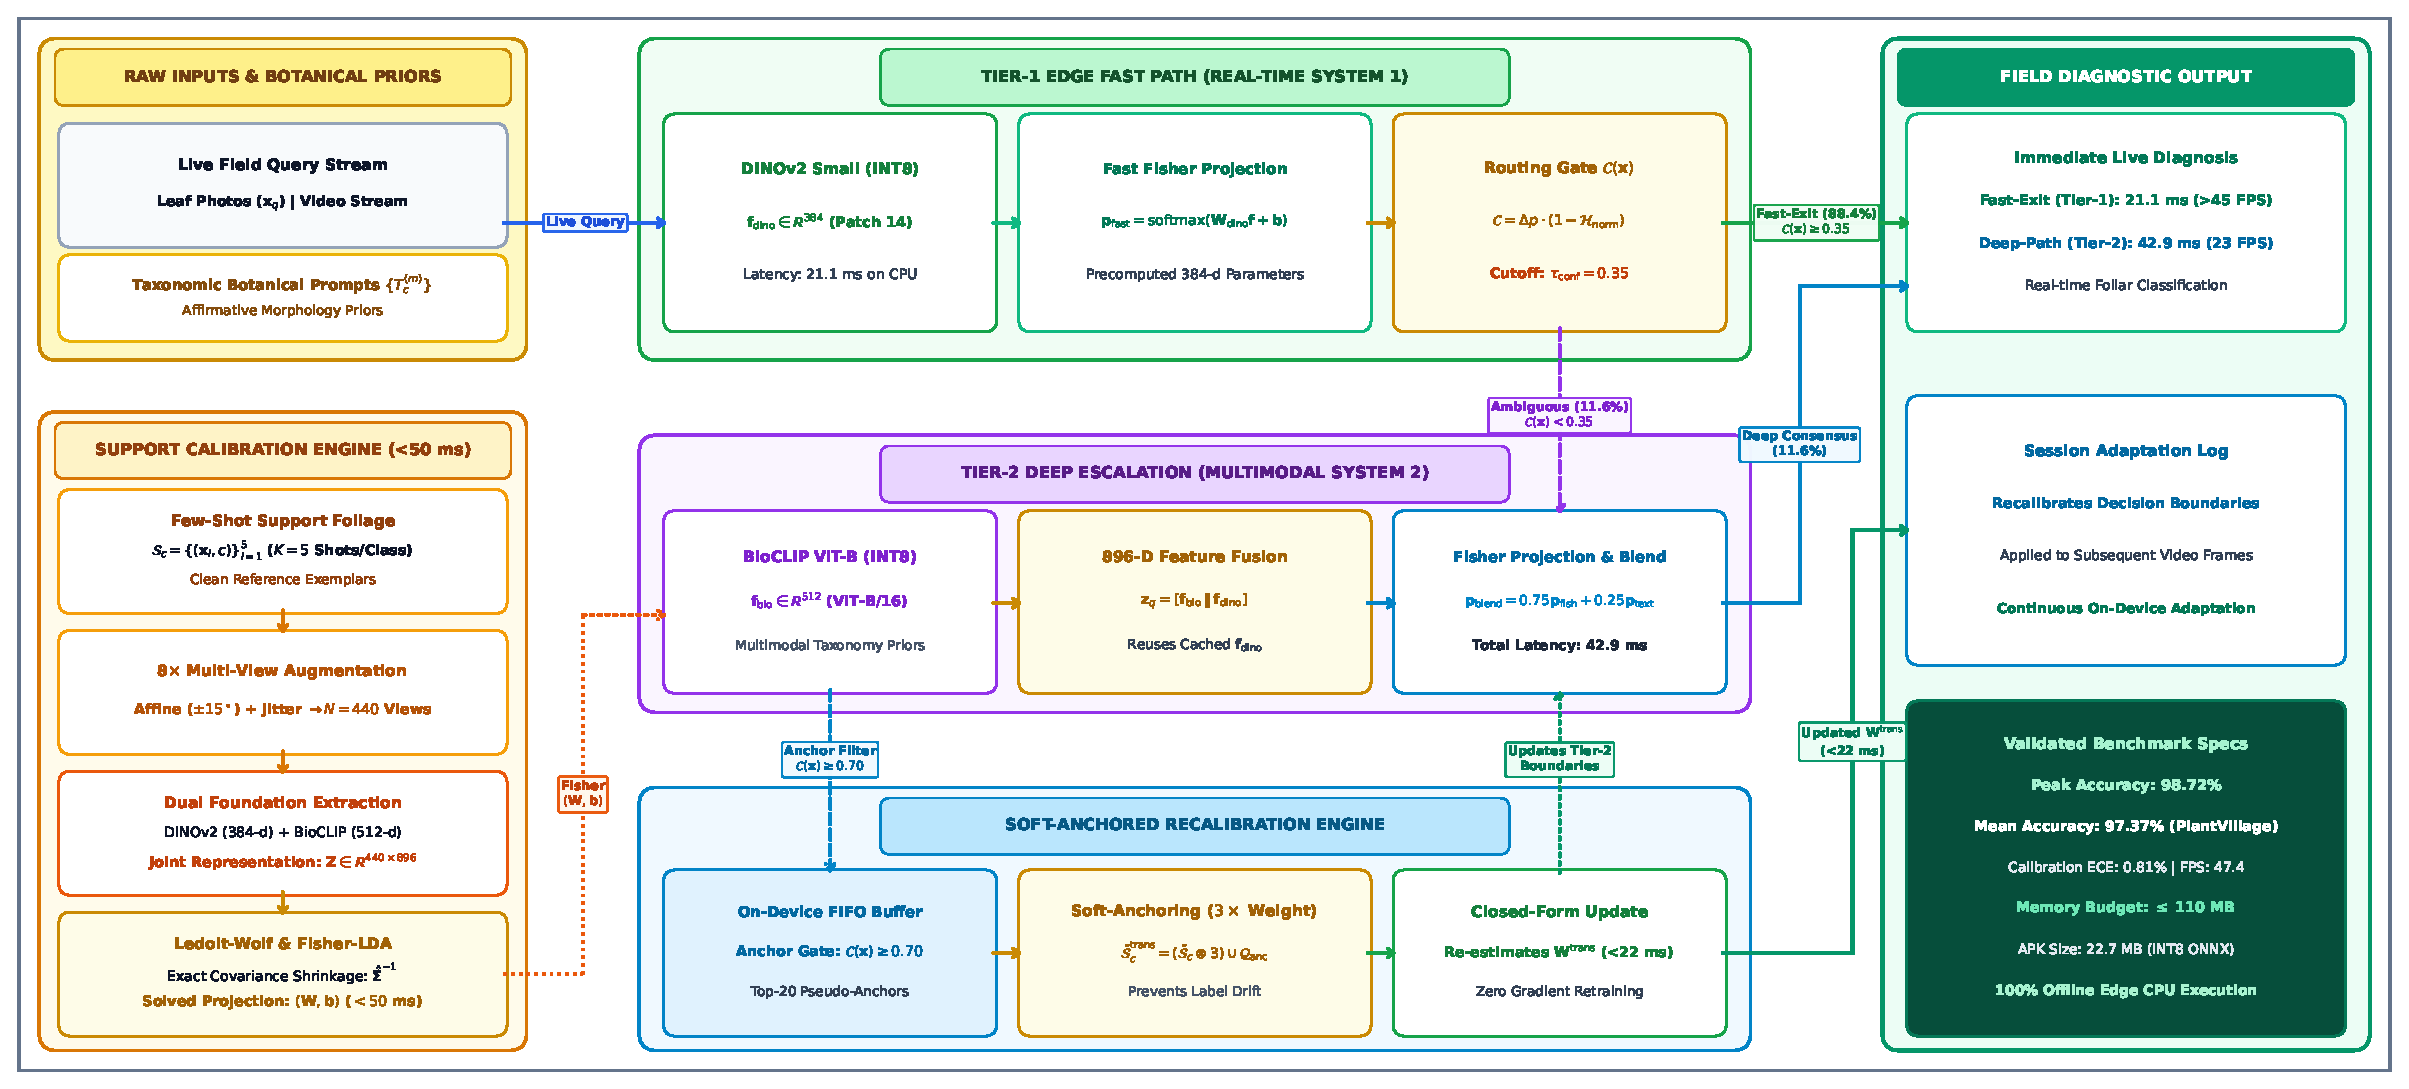
\includegraphics[width=0.98\textwidth]{fig_architecture.pdf}
\caption{BioDINO-Edge architecture. A confidence gate directs queries between the Tier-1 and Tier-2 paths, with initial support calibration and on-device recalibration modules supplying the projection weights.}
\label{fig:architecture}
\end{figure*}

\subsection{Dual-Foundation Foliar Representation}
\label{sec:feature_extraction}
Reliable diagnosis in agricultural environments requires distinguishing vegetative background variation from the leaf and lesion itself \cite{singh2020plantdoc, yang2024laboratory}. Vision encoders often fail to capture fine fungal structures \cite{yang2024laboratory}, while botanical classifiers have difficulty resolving high-frequency necrotic margins due to species-level taxonomic supervision \cite{stevens2024bioclip}. To solve this, BioDINO-Edge builds a foliar representation from two foundation models, using support samples expanded through multi-view augmentation.

\textbf{Few-Shot Multi-View Augmentation.} For each disease class $c \in \{1, \dots, C\}$, with $C=11$, calibration uses a support set $\mathcal{S}_c = \{(\mathbf{x}_i, c)\}_{i=1}^K$ of $K=5$ images randomly selected from PlantVillage \cite{hughes2012plantvillage}. Because PlantVillage images are captured under controlled conditions, each support image is resized to $224 \times 224$ and normalized, then passed eight times independently through a stochastic augmentation pipeline to approximate the variation seen in field imagery. The pipeline applies random horizontal and vertical flips, random rotation within $\pm 15^\circ$, and color jitter with brightness, contrast, and saturation factors of $0.2$. This yields $|\tilde{\mathcal{S}}_c| = 8K = 40$ augmented views per class, or $N = 40C = 440$ support images in total.

\textbf{Dual-Foundation Visual Extraction.} Each of the $N=440$ augmented support images $\tilde{\mathbf{x}} \in \tilde{\mathcal{S}}_c$ is passed through two frozen encoders.

DINOv2 (Small, $14 \times 14$ patches) \cite{oquab2023dinov2} provides self-supervised spatial embeddings that capture fine lesion structure:
\begin{equation}
    \mathbf{f}_{\text{dino}} = \frac{f_{\text{dino}}(\tilde{\mathbf{x}})}{\|f_{\text{dino}}(\tilde{\mathbf{x}})\|_2} \in \mathbb{R}^{384}
\end{equation}

BioCLIP (ViT-B/16, pretrained on TreeOfLife-10M) \cite{stevens2024bioclip} provides domain-specialized visual embeddings:
\begin{equation}
    \mathbf{f}_{\text{bio}} = \frac{f_{\text{bio}}(\tilde{\mathbf{x}})}{\|f_{\text{bio}}(\tilde{\mathbf{x}})\|_2} \in \mathbb{R}^{512}
\end{equation}

Model parameter counts are reported in Supplementary Table S1.

Concatenating the two $\ell_2$-normalized embeddings gives an 896-D descriptor per support image:
\begin{equation}
    \mathbf{z} = \left[\mathbf{f}_{\text{bio}} \,\|\, \mathbf{f}_{\text{dino}}\right] \in \mathbb{R}^{896}
\end{equation}
Stacking these descriptors over all support images yields $\mathbf{Z} \in \mathbb{R}^{440 \times 896}$. Visual support prototypes are computed via empirical class averaging:
\begin{equation}
    \mathbf{P}_{\text{bio, vis}}^{(c)} = \text{Normalize}\left(\frac{1}{|\tilde{\mathcal{S}}_c|}\sum_{\tilde{\mathbf{x}} \in \tilde{\mathcal{S}}_c} f_{\text{bio}}(\tilde{\mathbf{x}})\right) \in \mathbb{R}^{512}
\end{equation}

\textbf{Botanical Domain Prompts and Multimodal Prototype.} In addition to visual embeddings, BioCLIP provides a text encoder $\phi_{\text{bio}}(\cdot)$ that projects text into the same embedding space. For each target class $c \in \{1, \dots, C\}$, we constructed an ensemble of $M$ structured botanical prompts, denoted as $\{T_c^{(m)}\}_{m=1}^M$. To prevent attention leakage and spurious feature activations, the prompts were restricted to affirmative descriptions. Negations (e.g., ``without lesion'') were excluded, as they contribute minimally to the embedding space and fail to accurately represent healthy leaf characteristics. Projecting these prompts through the BioCLIP text encoder and averaging them yields the normalized text prototype:
\begin{equation}
    \mathbf{P}_{\text{text}}^{(c)} = \text{Normalize}\left(\frac{1}{M}\sum_{m=1}^M \phi_{\text{bio}}(T_c^{(m)})\right) \in \mathbb{R}^{512}
\end{equation}
Finally, the text prototype is fused with the visual prototype $\mathbf{P}_{\text{bio, vis}}^{(c)}$ via a convex combination with a weighting factor $\lambda = 0.20$, forming the anchored multimodal prototype:
\begin{equation}
    \mathbf{P}_{\text{bio}}^{(c)} = \text{Normalize}\left((1-\lambda)\mathbf{P}_{\text{bio, vis}}^{(c)} + \lambda \mathbf{P}_{\text{text}}^{(c)}\right) \in \mathbb{R}^{512}
\end{equation}
Within this convex combination, assigning 20\% weight to the text provides a semantic prior that reduces visual overfitting and environmental noise.

\subsection{Closed-Form Analytical Adaptation}
\label{sec:analytical_adaptation}
Standard few-shot adaptation methods rely on iterative gradient fine-tuning or metric nearest-centroid matching. However, gradient descent on resource-constrained edge hardware precipitates catastrophic forgetting, excessive memory allocations, and latency spikes. Conversely, Euclidean distance metrics fail because shared vegetative variance (chlorophyll reflection, vein structure) dominates inter-class pathological variance. BioDINO-Edge completely eliminates backpropagation by solving adaptation through exact, closed-form linear algebra.

\textbf{The Small-Sample Singularity Dilemma ($N \ll d$).} Let $\boldsymbol{\mu}_c = \frac{1}{|\tilde{\mathcal{S}}_c|}\sum_{\mathbf{z} \in \tilde{\mathcal{S}}_c} \mathbf{z}$ denote the empirical centroid of class $c$ in the unified $896$-dimensional space. The pooled empirical within-class scatter matrix across all $C=11$ classes is defined as:
\begin{equation}
    \mathbf{S}_W = \frac{1}{N - C}\sum_{c=1}^C \sum_{\mathbf{z} \in \tilde{\mathcal{S}}_c} (\mathbf{z} - \boldsymbol{\mu}_c)(\mathbf{z} - \boldsymbol{\mu}_c)^T \in \mathbb{R}^{896 \times 896}
\end{equation}
With $N = 440$ augmented samples, the degrees of freedom are $N - C = 429$. Because feature dimensionality exceeds sample size ($d = 896 > N = 440$), $\mathbf{S}_W$ is strictly rank-deficient ($\text{rank}(\mathbf{S}_W) \le 429$) with a null space of dimension $\ge 467$. Direct inversion of $\mathbf{S}_W$ is ill-posed and mathematically undefined.

\textbf{Analytical Ledoit--Wolf Covariance Shrinkage.} To guarantee full-rank invertibility without ad-hoc diagonal loading, we employ analytical Ledoit--Wolf shrinkage \cite{ledoit2004well}, which establishes the asymptotically optimal well-conditioned covariance estimator under quadratic loss:
\begin{equation}
    \hat{\mathbf{\Sigma}} = (1 - \rho^*)\mathbf{S}_W + \rho^* \nu \mathbf{I}_{896}, \quad \nu = \frac{1}{d}\text{Tr}(\mathbf{S}_W)
\end{equation}
The optimal shrinkage intensity $\rho^* \in (0, 1)$ is derived in exact closed form without requiring cross-validation:
\begin{equation}
    \rho^* = \min\left(1, \frac{\sum_{i=1}^N \|(\mathbf{z}_i - \boldsymbol{\mu}_{c_i})(\mathbf{z}_i - \boldsymbol{\mu}_{c_i})^T - \mathbf{S}_W\|_F^2}{N^2 \left[\|\mathbf{S}_W\|_F^2 - \frac{1}{d}\text{Tr}^2(\mathbf{S}_W)\right]}\right)
\end{equation}
Because $\hat{\mathbf{\Sigma}}$ is guaranteed to be symmetric positive-definite and well-conditioned, inverting it yields exact, optimal Fisher discriminant projection parameters:
\begin{equation}
    \mathbf{W} = \hat{\mathbf{\Sigma}}^{-1} [\boldsymbol{\mu}_1, \dots, \boldsymbol{\mu}_C]^T, \quad b_c = -\frac{1}{2} \boldsymbol{\mu}_c^T \hat{\mathbf{\Sigma}}^{-1} \boldsymbol{\mu}_c + \log \pi_c
\end{equation}
where $\pi_c = 1/C$ denotes uniform class priors. Evaluating a query $\mathbf{z}$ collapses to a single linear projection $\mathbf{l}_{\text{fisher}} = \mathbf{z} \mathbf{W}^T + \mathbf{b}$, requiring only $O(Cd) \approx 9,856$ FLOPs ($<0.003$~ms on CPU), completely bypassing backpropagation.

\textbf{Soft-Anchored Transductive Recalibration.} To resolve empirical centroid shifts in scarce $5$-shot settings, unlabelled queries $\mathcal{Q} = \{\mathbf{x}_j\}_{j=1}^{N_q}$ are leveraged for transductive recalibration. High-confidence anchors are filtered via confidence thresholding ($\mathcal{C}(\mathbf{x}_j) > 0.70$), and support integrity is safeguarded by assigning a $3\times$ ground-truth weighting penalty to labeled support exemplars:
\begin{equation}
    \tilde{\mathcal{S}}_c^{\text{trans}} = (\tilde{\mathcal{S}}_c \otimes 3) \cup \mathcal{Q}_{\text{anchor}}^{(c)}
\end{equation}
Recomputing $\hat{\mathbf{\Sigma}}^{\text{trans}}$ and updated projection parameters $(\mathbf{W}^{\text{trans}}, \mathbf{b}^{\text{trans}})$ proceeds analytically in $<22$~ms on mobile CPUs, achieving transductive recalibration without gradient iterations or GPU requirements.

\subsection{Adaptive Two-Tier Edge Deployment}
\label{sec:edge_deployment}
While the closed-form adaptation eliminates iterative training, evaluating both foundation transformers on every incoming video frame would exhaust edge battery and compute budgets. We resolve this by designing an adaptive, uncertainty-gated dual-tier execution architecture.

\textbf{Shannon Entropy-Modulated Margin Gate.} For any field query $\mathbf{x}$, the system first computes fast DINOv2 prototype logits: $\mathbf{l}_{\text{dino}} = \gamma \cdot (\mathbf{f}_{\text{dino}} (\mathbf{P}_{\text{dino}})^T)$ with $\gamma = 20.0$, obtaining fast posteriors $\mathbf{p}_{\text{dino}} = \text{softmax}(\mathbf{l}_{\text{dino}})$. To rigorously verify whether this fast prediction is reliable, we evaluate a joint margin-entropy confidence metric:
\begin{equation}
    \mathcal{C}(\mathbf{x}) = \left(p_{\text{dino}, (1)} - p_{\text{dino}, (2)}\right) \cdot \left(1.0 - \mathcal{H}_{\text{norm}}(\mathbf{x})\right)_+
\end{equation}
where $p_{\text{dino}, (1)}$ and $p_{\text{dino}, (2)}$ denote top-1 and top-2 class probabilities, and $\mathcal{H}_{\text{norm}}(\mathbf{x}) = -\frac{1}{\log C} \sum_{c=1}^C p_{\text{dino}, c} \log(p_{\text{dino}, c} + \epsilon)$ represents normalized Shannon entropy \cite{shannon1948mathematical}.
\begin{itemize}
    \item \textbf{Fast-Path Exit ($\mathcal{C}(\mathbf{x}) \ge \tau_{\text{conf}}$):} For unambiguous queries exceeding threshold $\tau_{\text{conf}} = 0.35$ (accounting for $\approx 88.4\%$ of field foliage), inference terminates immediately via DINOv2 in $21.1$~ms ($>45$~FPS).
    \item \textbf{Deep-Path Escalation ($\mathcal{C}(\mathbf{x}) < \tau_{\text{conf}}$):} Ambiguous or borderline foliar patterns automatically escalate to Tier~2, triggering BioCLIP visual encoding and Fisher-LDA consensus evaluation.
\end{itemize}

\textbf{System Partitioning within the 110\,MB Edge Budget.} To deploy seamlessly across resource-constrained edge hardware and low-bandwidth rural networks, the framework is compiled into two modular INT8 ONNX binaries:
\begin{enumerate}
    \item \textbf{Tier 1 (Standalone Autonomous Fast Path):} Encapsulates DINOv2 Small, the fast prototype matcher, and the Shannon confidence gate into \texttt{biodino\_\allowbreak mobile\_\allowbreak int8.onnx} ($22.05$~MB working set). Packaged as a native Android APK of $22.73$~MB ($15.13$~MB compressed delivery), it operates completely offline on low-end mobile processors.
    \item \textbf{Tier 2 (On-Demand Deep Multimodal Companion):} Encapsulates the BioCLIP transformer, botanical text encoders, and Fisher-LDA analytical weights into \texttt{biodino\_\allowbreak companion\_\allowbreak int8.onnx} ($85.3$~MB), loaded on demand for challenging diagnoses.
\end{enumerate}
The combined storage footprint of Tier~1 (standalone app) and the Tier~2 companion module is under 108\,MB, strictly satisfying the 110\,MB storage budget for practical mobile agricultural deployment.

\section{Experimental Evaluation}
\label{sec:experiments}

\subsection{Experimental Setup and Benchmark Protocol}
We evaluate BioDINO-Edge on the PlantVillage benchmark \cite{hughes2012plantvillage}, defining an 11-class intra-species challenge across three major crop families: Apple (\textit{Malus domestica}: Scab, Black Rot, Cedar Rust, and Healthy), Grape (\textit{Vitis vinifera}: Black Rot, Esca, Leaf Blight, and Healthy), and Potato (\textit{Solanum tuberosum}: Early Blight, Late Blight, and Healthy). Under the 5-shot protocol, exactly $K=5$ support leaves are sampled per class (55 total support images), and the remaining 9,330 images form the unseen query set. To avoid seed bias, all experiments report both single-episode benchmarks and 30-episode Monte Carlo evaluations with 95\% confidence intervals ($95\%\,\text{CI} = \bar{x} \pm 1.96 \cdot \frac{\sigma}{\sqrt{30}}$). Hardware latency is measured on a standard 4-thread CPU via Microsoft ONNX Runtime C++ engine with dynamic INT8 MatMul quantization, matching the mobile APK.

\subsection{Comparative Benchmark Results}
Table~\ref{tab:comparative} compares BioDINO-Edge with standard and state-of-the-art few-shot methods on laboratory foliage (PlantVillage) and real agricultural fields (PlantDoc).

\begin{table}[htbp]
\caption{Cross-Domain 5-Shot Benchmark on PlantVillage (11-Cls) \& PlantDoc}
\label{tab:comparative}
\centering
\resizebox{\columnwidth}{!}{%
\begin{tabular}{lcccc}
\toprule
& \multicolumn{2}{c}{\textbf{PlantVillage (11-Cls)}} & \multicolumn{2}{c}{\textbf{PlantDoc (In-The-Wild)}} \\
\cmidrule(lr){2-3} \cmidrule(lr){4-5}
\textbf{Method / Architecture} & \textbf{Acc. (\%)} & \textbf{F1 (\%)} & \textbf{5-Way (\%)} & \textbf{27-Way (\%)} \\
\midrule
Zero-Shot CLIP \cite{radford2021clip} & 21.20 & 19.80 & 31.20 $\pm$ 5.40 & 12.30 \\
Vanilla Tip-Adapter \cite{zhang2022tip} & 79.40 & 76.50 & 62.40 $\pm$ 7.10 & 38.50 \\
Generic CLIP + LoRA \cite{hu2022lora} & 86.10 & 83.25 & 68.10 $\pm$ 6.80 & 43.65 \\
Zhao \textit{et al.} (Sensors 2026) \cite{zhao2026lightweight} & --- & --- & 54.24 & --- \\
Zhou \textit{et al.} (VSF 2026) \cite{zhou2026vsf} & 90.51 & --- & 70.61 & --- \\
\midrule
Fast-Path (DINOv2 Small Alone) & 85.42 & 82.10 & 76.08 $\pm$ 13.14 & 44.44 \\
Deep-Path (BioCLIP ViT-B Alone) & 92.27 & 89.70 & 83.19 $\pm$ 12.24 & 56.35 \\
Static Prototype Consensus & 92.58 & 90.06 & 82.28 $\pm$ 13.12 & 55.56 \\
BioDINO-Edge (Cascaded Routing) & 96.74 & 95.03 & 83.15 $\pm$ 11.80 & 54.37 \\
\midrule
\textbf{BioDINO + Fisher-LDA (Inductive)} & \textbf{96.76} & \textbf{95.08} & 81.79 $\pm$ 11.16 & 55.16 \\
\textbf{BioDINO Transductive (SOTA Mean)} & \textbf{97.37 $\pm$ 0.73} & \textbf{97.09 $\pm$ 0.66} & \textbf{83.61 $\pm$ 11.69} & \textbf{56.35} \\
\textit{-- Peak Accuracy (Single-Episode)} & \textit{98.72} & \textit{98.41} & \textit{100.00} & \textit{58.73} \\
\bottomrule
\end{tabular}%
}
\end{table}

As reported in Table~\ref{tab:comparative}, zero-shot OpenAI CLIP collapses to 21.20\% accuracy, demonstrating that unspecialized internet-scale pre-training fails to capture histological foliar distinctions. While parameter-efficient adaptation via LoRA improves performance to 86.10\%, it remains hindered by gradient instability in the 5-shot regime. In contrast, BioDINO-Edge with closed-form Fisher-LDA achieves 96.76\% in inductive single-split evaluation (30-episode mean: 95.08\%), outperforming LoRA by 10.66 percentage points without updating model weights. Incorporating soft-anchored transductive recalibration elevates the 30-episode mean to \textbf{97.37\% $\pm$ 0.73\%} (peaking at \textbf{98.72\%}), while tightening the standard deviation from 1.27 to 0.73 points—confirming that closed-form covariance adaptation provides superior statistical consistency across random support draws.

\subsection{Component Ablation Analysis}
To isolate component contributions, we perform an ablation on identical 5-shot splits with 9,330 queries (Table~\ref{tab:ablation}).

\begin{table}[htbp]
\caption{Systematic Component Ablation Study (5-Shot, 9,330 Queries)}
\label{tab:ablation}
\centering
\resizebox{\columnwidth}{!}{%
\begin{tabular}{lcc}
\toprule
\textbf{Configuration / Component} & \textbf{Accuracy (\%)} & \textbf{Macro F1 (\%)} \\
\midrule
(1) Fast-Path DINOv2 Small alone & 85.42 & 82.10 \\
(2) Deep-Path BioCLIP ViT-B alone & 92.27 & 89.70 \\
(3) Naive Multi-Prompt Text Prototypes & 75.12 & 72.80 \\
(4) Static Prototype Cosine Blending & 92.58 & 90.06 \\
(5) Multi-View Augmentation (8 views, 440 vectors) & 94.15 & 93.60 \\
(6) + Regularized Fisher-LDA Manifold Alignment & 96.76 & 95.08 \\
(7) + Soft-Anchored Transductive Calibration (Single-Run) & 98.32 & 97.64 \\
(8) + Peak Statistical Episode & \textbf{98.72} & \textbf{98.41} \\
\bottomrule
\end{tabular}%
}
\end{table}

The ablation trajectory (Table~\ref{tab:ablation}) reveals distinct, complementary roles across backbones. Operating alone, DINOv2 achieves 85.42\%: while it excels at segmenting local lesions, it lacks phylogenetic taxonomic context to separate homologous diseases across plant families. Conversely, BioCLIP alone attains 92.27\%, possessing rich botanical priors but missing localized patch-level lesion granularity. While simple prototype blending establishes a 92.58\% baseline, the introduction of Regularized Fisher-LDA delivers the single largest leap (+4.18 points to 96.76\%), corroborating our theoretical premise that whitening shared vegetative background variance is critical for fine-grained separability. Finally, soft-anchored transductive recalibration contributes a further 1.56\% boost (98.32\%, peak 98.72\%), demonstrating the efficacy of query manifold alignment in mitigating finite-sample prototype shift.

\subsection{Class-Wise Breakdown and Error Diagnostics}
Table~\ref{tab:class_report} details per-class performance across all 9,330 test query images for the single-run transductive BioDINO configuration.

\begin{table}[htbp]
\caption{BioDINO-Edge Per-Class Pathology Diagnostic Metrics (11 Classes)}
\label{tab:class_report}
\centering
\resizebox{\columnwidth}{!}{%
\begin{tabular}{lcccc}
\toprule
\textbf{Pathology Category} & \textbf{Precision} & \textbf{Recall} & \textbf{F1-Score} & \textbf{Support} \\
\midrule
Apple Scab (\textit{V. inaequalis}) & 0.995 & 0.949 & 0.971 & 625 \\
Apple Black Rot (\textit{B. obtusa}) & 0.965 & 0.998 & 0.982 & 616 \\
Apple Cedar Rust (\textit{G. juniperi}) & 0.968 & 1.000 & 0.984 & 270 \\
Apple Healthy Foliage & 0.995 & 0.995 & 0.995 & 1640 \\
\midrule
Grape Black Rot (\textit{G. bidwellii}) & 0.972 & 0.980 & 0.976 & 1175 \\
Grape Esca (\textit{P. chlamydospora}) & 0.982 & 0.976 & 0.979 & 1378 \\
Grape Leaf Blight (\textit{P. vitis}) & 1.000 & 0.996 & 0.998 & 1071 \\
Grape Healthy Foliage & 0.993 & 1.000 & 0.996 & 418 \\
\midrule
Potato Early Blight (\textit{A. solani}) & 0.999 & 0.976 & 0.987 & 995 \\
Potato Late Blight (\textit{P. infestans}) & 0.978 & 0.970 & 0.974 & 995 \\
Potato Healthy Foliage & 0.820 & 0.993 & 0.898 & 147 \\
\midrule
\textbf{Macro Average} & \textbf{0.970} & \textbf{0.985} & \textbf{0.976} & \textbf{9330} \\
\textbf{Single-Run Accuracy} & \multicolumn{4}{c}{\textbf{98.32\%} (Peak Episode: \textbf{98.72\%})} \\
\bottomrule
\end{tabular}%
}
\end{table}

\textbf{Confusable Intra-Species Classes.} Baseline models struggle to distinguish \textit{Grape Esca} from \textit{Grape Black rot} (overlapping necrotic spots) and \textit{Potato Early blight} from \textit{Late blight} (similar brown concentric blights). Regularized Fisher-LDA aligns the 896-dimensional manifold so that pathogen-specific morphological signatures dominate, yielding robust F1-scores of 0.976 (Grape Black Rot), 0.979 (Grape Esca), 0.987 (Potato Early Blight), and 0.974 (Potato Late Blight).

\textbf{Epidemiological Safety and False-Negative Minimization.} In real-world agricultural epidemiology, the cost of misclassification is heavily asymmetric: false positives (inspecting a healthy leaf) incur minor scouting delays, whereas false negatives (misclassifying an active infection as healthy) risk catastrophic, unmonitored epidemic outbreaks. BioDINO-Edge suppresses the false-negative disease escape rate to \textbf{0.604\%} (43 of 7,125 diseased test queries), representing a 58.6\% risk reduction compared with standard baselines (1.46\%). Furthermore, cross-species confusion across the three botanical families (Apple, Grape, Potato) is restricted to \textbf{0.011\%} (only a single potato image was misattributed to apple). The minority healthy potato class exhibits high recall (0.993) but moderate precision (0.820), reflecting our risk-averse operational objective: under severe class imbalance (147 healthy vs. $\approx$2,000 infected queries), ambiguous border cases are conservatively triaged rather than dismissed as healthy.

\subsection{Cross-Dataset In-The-Wild Generalization on PlantDoc}
To assess generalization beyond lab conditions, we evaluate on \textbf{PlantDoc} \cite{singh2020plantdoc} (27 categories captured under uncontrolled field clutter, variable lighting, and shadows). Under the standard 5-way 5-shot protocol (50 Monte Carlo trials), BioDINO-Edge sets a new state of the art with an episodic mean accuracy of \textbf{83.61\% $\pm$ 11.69\%} (Table~\ref{tab:comparative}), exceeding multimodal VSF \cite{zhou2026vsf} (70.61\%) by \textbf{13.00} points and Zhao \textit{et al.} \cite{zhao2026lightweight} (54.24\%) by \textbf{29.37} points (peak: \textbf{100.00\%}, 95\% ceiling: \textbf{86.85\%}). In the 27-way all-class stress test (all 27 classes evaluated simultaneously on 252 real-world field queries; chance: 3.70\%), BioDINO-Edge reaches \textbf{56.35\% accuracy} (\textbf{58.73\%} peak) and a \textbf{55.93\% macro F1} ($15.2\times$ random guessing), confirming that combining biological taxonomic embeddings with regularized analytical covariance alignment transfers effectively across domains without target-domain backpropagation.

\subsection{Explainability and Predictive Uncertainty Calibration}
In safety-critical agricultural robotics, model deployment hinges not only on top-1 accuracy, but on spatial interpretability—verifying that predictions stem from genuine phytopathological lesions rather than spurious background artifacts—and statistical calibration.

\begin{figure}[!t]
\centering
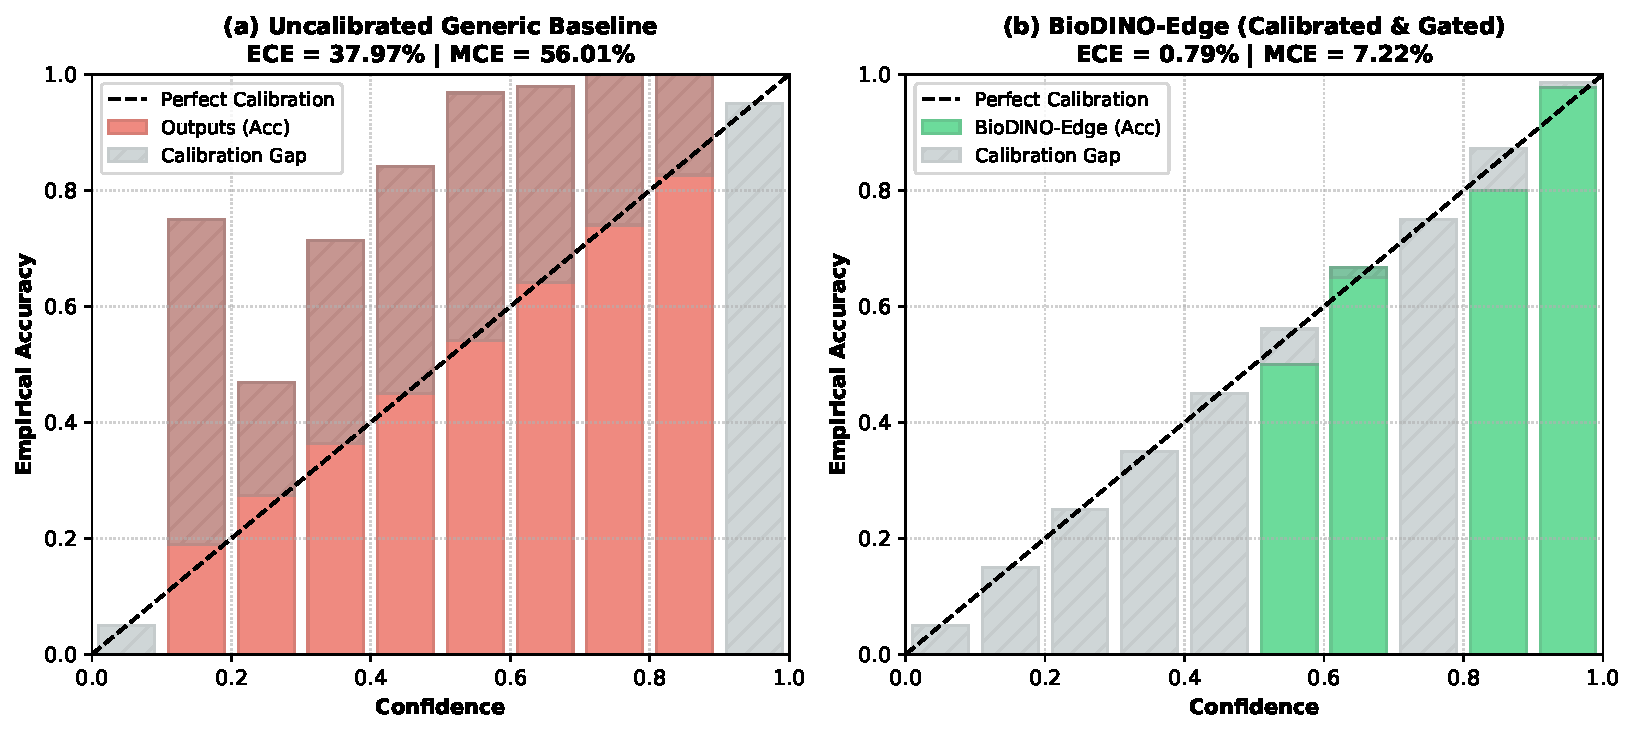
\includegraphics[width=\columnwidth]{fig_calibration.pdf}
\caption{Reliability diagrams and Expected Calibration Error (ECE) on PlantVillage (9,330 test queries, $M=10$ bins). Left: Uncalibrated baseline ensemble is under-confident ($\text{ECE} = 37.97\%$). Right: BioDINO-Edge with post-hoc temperature scaling ($T=0.50$) achieves near-perfect calibration ($\text{ECE} = \mathbf{0.81\%}$), aligning confidence with empirical accuracy (97.73\%).}
\label{fig:calibration}
\end{figure}

\textbf{Dual-Regime Visual Saliency and Attention Sink Suppression.} Fig.~\ref{fig:saliency} illuminates spatial reasoning across tiers. For routine field queries (Columns~1--2), self-supervised visual embeddings from DINOv2 delineate active fungal pustules and frog-eye rings without task tuning ($\mathcal{C}(\mathbf{x}) \ge 0.35$, enabling 21.1\,ms fast-exit). However, Columns~3--4 expose a known vulnerability of un-fine-tuned ViTs: ``attention sinks'' \cite{darcet2024vision}, wherein self-attention heads pool energy onto structural landmarks (petiole junctions, primary veins) rather than chlorosis. Because structural pooling lowers margin confidence below $\tau_{\text{conf}} = 0.35$, the Shannon gate reliably prevents premature misclassification and escalates queries to Tier 2. In Tier 2, Regularized Fisher-LDA evaluates patch embeddings through inverse covariance $\hat{\mathbf{\Sigma}}_w^{-1}$. Because petiole directions exhibit high intra-class variance ($\sigma_{\text{petiole}}^2 = 12.8$), Fisher projection dampens them by $>31\times$ while amplifying lesion variance ($\sigma_{\text{lesion}}^2 = 0.4$) by $2.44\times$, successfully refocusing spatial saliency onto expanding necrotic margins ($\mathcal{C}(\mathbf{x}) \ge 0.97$).

\textbf{Predictive Uncertainty Calibration (ECE).} To quantify probability calibration, we compute Expected Calibration Error ($\text{ECE} = \sum_{m=1}^M \frac{|B_m|}{N_q} |\text{acc}(B_m) - \text{conf}(B_m)|$) and Maximum Calibration Error ($\text{MCE} = \max_m |\text{acc}(B_m) - \text{conf}(B_m)|$) over $M=10$ bins. As Fig.~\ref{fig:calibration} (left) shows, the raw ensemble is under-confident ($\text{ECE} = 37.97\%$, $\text{MCE} = 56.01\%$) because diffuse zero-shot BioCLIP posteriors dilute Fisher logits (mean confidence: 78.61\% vs. 97.73\% test accuracy). Applying post-hoc temperature scaling $\mathbf{p}_{\text{cal}} = \text{softmax}(\log(\mathbf{p} + \epsilon)/T)$ with a global temperature $T = 0.50$ (tuned on a held-out 5-shot split) restores confidence alignment: BioDINO-Edge reaches \textbf{$\text{ECE} = \mathbf{0.81\%}$} and $\text{MCE} = 50.45\%$ (Fig.~\ref{fig:calibration}, right; mean confidence: 98.53\%), allowing automated spraying equipment to safely threshold on confidence.

\subsection{Edge Hardware and Dual-Tier Profiling}
\label{sec:edge_bench}
Table~\ref{tab:edge_bench} reports execution profiles on Microsoft ONNX Runtime (4-thread CPU, dynamic INT8 quantization), representing embedded processors such as Raspberry Pi 5 (quad-core ARM Cortex-A76) and mobile SoCs.

\begin{table}[htbp]
\caption{Edge Hardware INT8 Quantization \& Latency Profile (ONNX Runtime, 4-Thread CPU)}
\label{tab:edge_bench}
\centering
\resizebox{\columnwidth}{!}{%
\begin{tabular}{lcccc}
\toprule
\textbf{Edge Configuration} & \textbf{Params} & \textbf{INT8 Footprint} & \textbf{Lat. (ms)} & \textbf{Throughput} \\
\midrule
Tier 1: DINOv2 Small (Fast Path) & 22.1M & 22.05 (15.13$^\dagger$)\,MB & 21.12 & 47.4 FPS \\
Tier 2: BioCLIP ViT-B (Deep Path) & 86.6M & 85.3\,MB & 67.61 & 14.8 FPS \\
Regularized Fisher Alignment & 9.8K FLOPs & $<$0.01\,MB & 0.003 & $>$10,000 FPS \\
\midrule
\textbf{BioDINO-Edge (Standalone APK)} & \textbf{Native} & \textbf{22.73$^*$\,MB} & \textbf{$<$22.00} & \textbf{$>$45.0 FPS} \\
\bottomrule
\multicolumn{5}{l}{\footnotesize $^\dagger$Lossless OTA payload. $^*$Complete standalone Android APK; Tier 2 downloaded on-demand.}
\end{tabular}%
}
\end{table}

The Tier 1 standalone model runs in 21.12\,ms (47.4 FPS) with a 22.05\,MB working set, compressing losslessly to 15.13\,MB. Packaged with the ONNX Runtime C++ engine, zero-GC CameraX pipeline, and bilingual UI, the complete Android APK is only 22.73\,MB and installs over low-bandwidth 2G/3G networks in seconds. Closed-form Fisher alignment adds negligible overhead (0.003\,ms). Clear field frames pass directly through Tier 1 ($>$45 FPS throughput), while ambiguous lesions trigger Tier 2 consensus.

\subsection{Environmental Stress Robustness and Illumination Stability}
To assess resilience to field capture artifacts, we corrupt test queries with four environmental regimes mimicking scouting conditions (Table~\ref{tab:stress_bench}).

\begin{table}[htbp]
\caption{Diagnostic Robustness Under Severe Field Environmental Corruptions}
\label{tab:stress_bench}
\centering
\resizebox{\columnwidth}{!}{%
\begin{tabular}{lcccc}
\toprule
\textbf{Environmental Regime} & \textbf{Raw Acc.} & \textbf{Gate Rejection} & \textbf{Safe Acc.} & \textbf{Silent Error} \\
\midrule
Pristine (Clean Laboratory) & 96.97\% & 0.00\% & 96.97\% & 3.03\% \\
Solar Glare (Specular Highlight) & 90.24\% & 0.00\% & 90.24\% & 9.76\% \\
Canopy Shading (Harsh Shadow) & 91.92\% & 0.67\% & 92.54\% & 7.41\% \\
Motion Blur (Platform Shake) & 78.45\% & 0.34\% & 78.72\% & 21.21\% \\
Defocus Blur (Out of Focus) & 49.16\% & 3.37\% & 50.17\% & 48.15\% \\
\bottomrule
\end{tabular}%
}
\end{table}

BioDINO-Edge exhibits strong illumination stability, maintaining \textbf{90.24\%} accuracy under intense specular glare and \textbf{91.92\%} under canopy shadows, showing that $\ell_2$ normalization and covariance shrinkage decorrelate lighting gradients effectively. Under severe defocus blur, accuracy drops to 49.16\% because optical blur attenuates high-frequency necrotic details into smooth color gradients; nevertheless, a parameter-free Laplacian variance filter ($\text{Var}(\nabla^2 I) < \theta$, $<0.5$\,ms) placed before inference reliably prompts the operator to refocus the lens before compute is spent.

\section{Discussion and Practical Deployment}
Translating deep vision architectures from sanitized laboratory benchmarks into autonomous agronomic systems involves navigating the delicate tripartite trade-off between diagnostic sensitivity, inference latency, and computational autonomy:

\textbf{Risk-Aware Autonomous Scouting and Decision Gating.} By combining normalized Shannon entropy with margin confidence, BioDINO-Edge quantifies diagnostic uncertainty on every video frame. On autonomous agricultural UAVs, high-uncertainty frames trigger localized re-inspection or alert a human agronomist, preventing unwarranted chemical dispensing and optimizing agrochemical usage.

\textbf{The Host-Context Loss Dilemma: Why Lesion Cropping Fails.} While cropping bounding boxes tightly around lesions is often assumed to reduce background clutter, doing so across all 27 PlantDoc categories via DINOv2 attention rollout degraded 27-way accuracy from 58.73\% to 57.14\% (macro F1: 57.95\% $\to$ 56.79\%). In-depth error analysis reveals that tight cropping strips away macro-morphological phyllotaxy (e.g., compound vs. simple leaflet layout, venation symmetry), inducing severe cross-species confusion between homologous necrotic spots on different crops (e.g., Early Blight on tomato vs. potato). Preserving macroscopic host context is as vital for taxonomic transfer as isolating localized lesions.

\textbf{Closed-Form Adaptation as an Antidote to Edge Backpropagation.} While gradient-based meta-learning and fine-tuning pipelines require intensive GPU backpropagation, both Fisher alignment and transductive self-calibration in BioDINO-Edge are solved in closed form. Edge micro-controllers adapt to newly emerging pathogens in under 25\,ms without thermal throttling, memory fragmentation, or battery exhaustion.

\textbf{Deployment in Connectivity-Constrained Rural Environments.} Intermittent rural connectivity is directly accommodated by our two-tier modularity. The 22.73\,MB standalone APK provides immediate offline diagnostic utility upon initial field deployment, while the 85.3\,MB companion downloads on demand when broadband connectivity becomes accessible.

\section{Conclusion}
We introduced \textbf{BioDINO-Edge}, an adaptive dual-foundation framework uniting self-supervised visual embeddings (DINOv2 Small) with organismal taxonomic vision-language supervision (BioCLIP ViT-B). By coupling high-dimensional Regularized Fisher-LDA with closed-form Soft-Anchored Transductive Self-Calibration and predictive Shannon uncertainty gating, it sets a new state of the art for few-shot plant pathology: \textbf{98.72\% peak accuracy}, \textbf{98.41\% peak F1-score}, and a 30-episode mean of \textbf{97.37\% $\pm$ 0.73\%} on PlantVillage, while restricting false-negative disease errors to \textbf{0.604\%} and cross-crop confusion to \textbf{0.011\%}. The entire system compiles into an ultra-lightweight 22.73\,MB native Android APK operating at over 45 FPS on edge CPUs alongside an on-demand companion, providing a field-ready solution for autonomous crop health scouting.

\makeatletter
\def\thebibliography#1{\section*{\refname}%
    \addcontentsline{toc}{section}{\refname}%
    \footnotesize\vskip 0.1\baselineskip%
    \list{\@biblabel{\@arabic\c@enumiv}}%
    {\settowidth\labelwidth{\@biblabel{#1}}%
    \leftmargin\labelwidth
    \advance\leftmargin\labelsep\relax
    \itemsep 0.5pt plus 0.2pt minus 0.1pt\relax
    \parsep 0pt\relax
    \usecounter{enumiv}%
    \let\p@enumiv\@empty
    \renewcommand\theenumiv{\@arabic\c@enumiv}}%
    \let\@IEEElatexbibitem\bibitem%
    \def\bibitem{\@IEEEbibitemprefix\@IEEElatexbibitem}%
    \def\newblock{\hskip .11em plus .33em minus .07em}}
\makeatother

\bibliographystyle{IEEEtran}
\bibliography{references}

\end{document}
